\documentclass[tikz,border=3mm]{standalone}
\usetikzlibrary{arrows.meta, positioning, shapes.geometric, fit}

\begin{document}
\sffamily
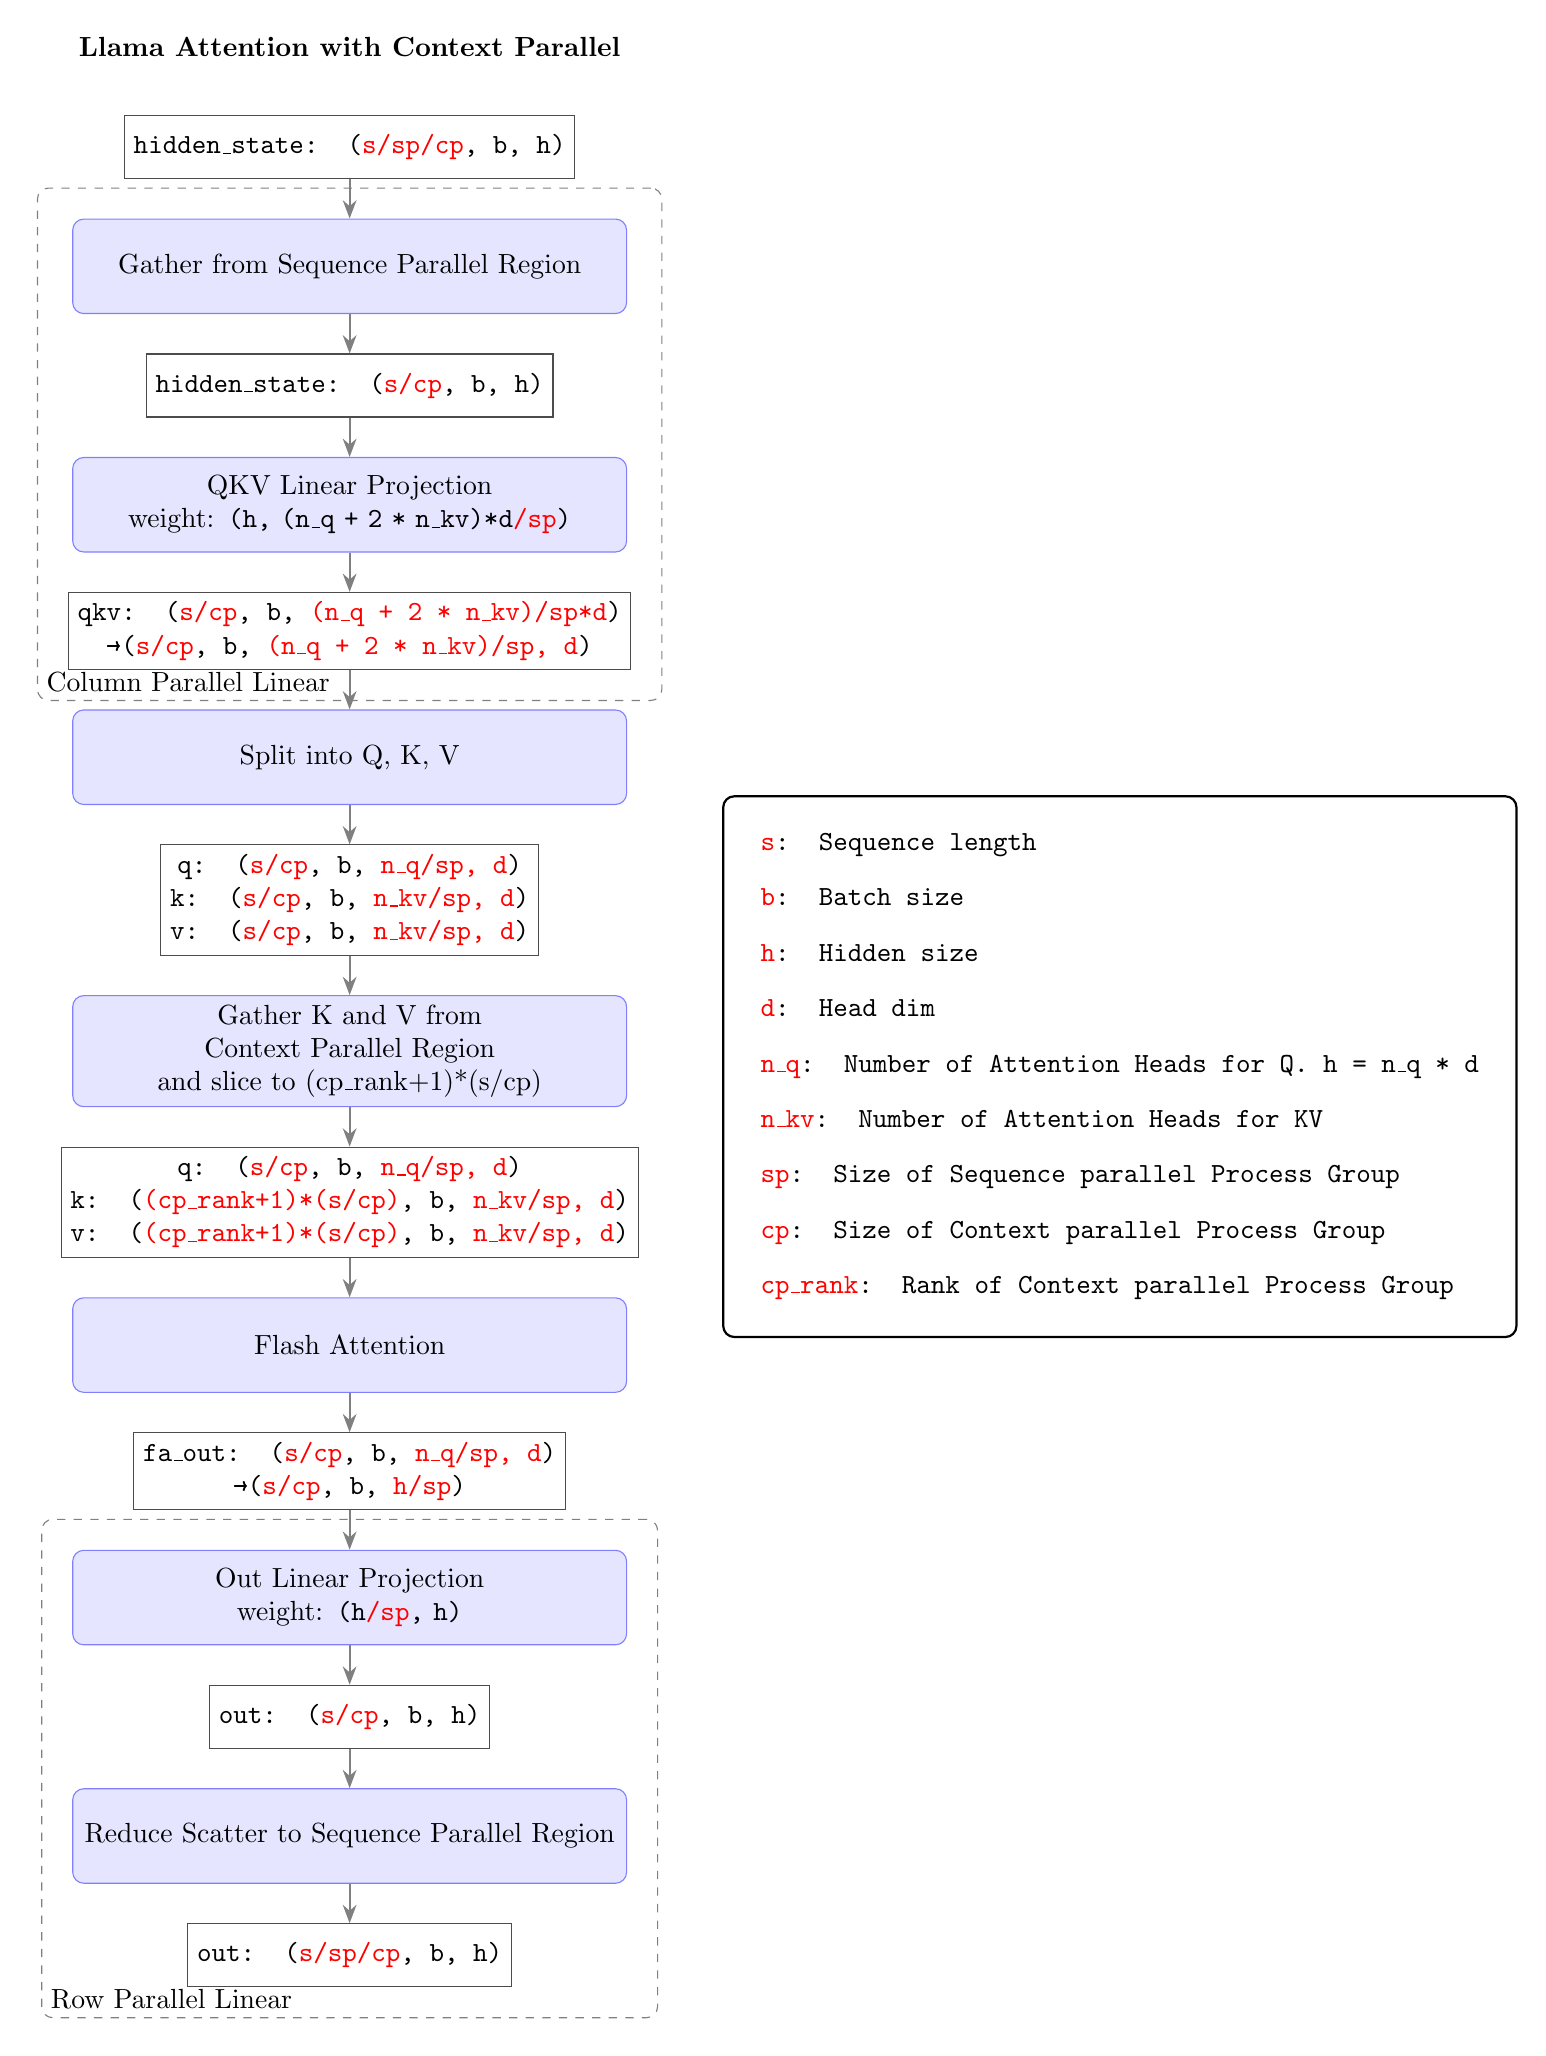
\begin{tikzpicture}[
    node distance=5mm,
    operation/.style={rectangle, draw=blue!50, fill=blue!10, rounded corners, minimum width=7cm, minimum height=1.2cm, text width=6.8cm, align=center},
    shapebox/.style={rectangle, draw=black!70, fill=white, minimum width=2.5cm, minimum height=0.8cm, font=\ttfamily, align=center},
    arrow/.style={-Stealth, thick, draw=black!50},
    groupbox/.style={draw=black!50, dashed, rounded corners, inner sep=11pt},
    outerbox/.style={},
    legendbox/.style={draw=black, thick, rounded corners, inner sep=10pt}
]

% 初始输入
\node[shapebox] (input) {hidden\_state: (\textcolor{red}{s/sp/cp}, b, h)};

% AG
\node[operation, below=of input] (ag) {Gather from Sequence Parallel Region};
\node[shapebox, below=of ag] (ag-output) {hidden\_state: (\textcolor{red}{s/cp}, b, h)};

% proj
\node[operation, below=of ag-output] (proj) {QKV Linear Projection \\ weight: \texttt{(h, (n\_q + 2 * n\_kv)*d\textcolor{red}{/sp})}};
\node[shapebox, below=of proj] (proj-output) {qkv: (\textcolor{red}{s/cp}, b, \textcolor{red}{(n\_q + 2 * n\_kv)/sp*d}) \\ \textrightarrow (\textcolor{red}{s/cp}, b, \textcolor{red}{(n\_q + 2 * n\_kv)/sp, d})};

% QKV split
\node[operation, below=of proj-output] (split) {Split into Q, K, V};
\node[shapebox, below=of split] (split-output) {q: (\textcolor{red}{s/cp}, b, \textcolor{red}{n\_q/sp, d}) \\ k: (\textcolor{red}{s/cp}, b, \textcolor{red}{n\_kv/sp, d}) \\ v: (\textcolor{red}{s/cp}, b, \textcolor{red}{n\_kv/sp, d})};

% KV gather
\node[operation, below=of split-output] (kvgather) {Gather K and V from Context Parallel Region \\ and slice to (cp\_rank+1)*(s/cp)};
\node[shapebox, below=of kvgather] (kvgather-output) {q: (\textcolor{red}{s/cp}, b, \textcolor{red}{n\_q/sp, d}) \\ k: (\textcolor{red}{(cp\_rank+1)*(s/cp)}, b, \textcolor{red}{n\_kv/sp, d}) \\ v: (\textcolor{red}{(cp\_rank+1)*(s/cp)}, b, \textcolor{red}{n\_kv/sp, d})};

% fa
\node[operation, below=of kvgather-output] (fa) {Flash Attention};
\node[shapebox, below=of fa] (fa-output) {fa\_out: (\textcolor{red}{s/cp}, b, \textcolor{red}{n\_q/sp, d})\\\textrightarrow (\textcolor{red}{s/cp}, b, \textcolor{red}{h/sp})};

% oproj
\node[operation, below=of fa-output] (oproj) {Out Linear Projection \\ weight: \texttt{(h\textcolor{red}{/sp}, h)}};
\node[shapebox, below=of oproj] (oproj-output) {out: (\textcolor{red}{s/cp}, b, h)};

% rs
\node[operation, below=of oproj-output] (rs) {Reduce Scatter to Sequence Parallel Region};
\node[shapebox, below=of rs] (rs-output) {out: (\textcolor{red}{s/sp/cp}, b, h)};

% 连接箭头
\draw[arrow] (input) -- (ag);
\draw[arrow] (ag) -- (ag-output);
\draw[arrow] (ag-output) -- (proj);
\draw[arrow] (proj) -- (proj-output);
\draw[arrow] (proj-output) -- (split);
\draw[arrow] (split) -- (split-output);
\draw[arrow] (split-output) -- (kvgather);
\draw[arrow] (kvgather) -- (kvgather-output);
\draw[arrow] (kvgather-output) -- (fa);
\draw[arrow] (fa) -- (fa-output);
\draw[arrow] (fa-output) -- (oproj);
\draw[arrow] (oproj) -- (oproj-output);
\draw[arrow] (oproj-output) -- (rs);
\draw[arrow] (rs) -- (rs-output);

% 添加分组框
\node[groupbox, fit=(ag) (ag-output) (proj) (proj-output), label={[anchor=south west]south west:Column Parallel Linear}] (agprojbox) {};
\node[groupbox, fit=(oproj) (oproj-output) (rs) (rs-output), label={[anchor=south west]south west:Row Parallel Linear}] (oprojrsbox) {};

% 添加外框
\node[outerbox, fit=(input) (rs-output) (agprojbox) (oprojrsbox)] (outerbox) {};

% 维度说明
\node[anchor=west, align=left, execute at begin node=\setlength{\baselineskip}{2em}\ttfamily] at ([xshift=1cm]outerbox.east) (legend) {
\baselineskip=20pt
\textcolor{red}{s}: Sequence length\\
\textcolor{red}{b}: Batch size\\
\textcolor{red}{h}: Hidden size\\
\textcolor{red}{d}: Head dim\\
\textcolor{red}{n\_q}: Number of Attention Heads for Q. h = n\_q * d\\
\textcolor{red}{n\_kv}: Number of Attention Heads for KV\\
\textcolor{red}{sp}: Size of Sequence parallel Process Group\\
\textcolor{red}{cp}: Size of Context parallel Process Group\\
\textcolor{red}{cp\_rank}: Rank of Context parallel Process Group
};
\node[legendbox, fit=(legend)] {};

% 标题
\node[above=5mm of outerbox, font=\bfseries] {Llama Attention with Context Parallel};
\end{tikzpicture}
\end{document}